\documentclass{article}
\usepackage[french]{babel}
\usepackage[utf8]{inputenc}

\usepackage{graphicx}
\graphicspath{{image/}}
\begin{document}
\title{Cours de Shiny \\ Création d'applications interactives avec R}

\author{François}
\maketitle

\section{Détails techniques}
L'application doit être rangée dans un dossier. Dans ce dossier il faut avoir :\\
\begin{itemize}
\item
ui.R le fichier de définition de l'interface. Il début avec du code qui ressemble à : 
\begin{verbatim}
shinyUI(fluidPage(
  titlePanel("My Shiny App"),
  sidebarLayout(
    sidebarPanel(
      h2("Installation"),
\end{verbatim}
\item
server.R le fichier qui execute le code
\end{itemize}
On lance ensuite l'application en utilisant :
\begin{verbatim}
library("shiny")
runApp("FolderName")
\end{verbatim}
\section{Widgets}
Pour créer des widgets, qui permettent à l'utilisateur de rentrer des informations, choisir des dates, etc... il faut utiliser au sein d'un appel à une fonction de type \verb!*Panel! des appels à des fonctions de type \verb!*Input! .
Par exemple :
\begin{verbatim}
shinyUI(fluidPage(
        titlePanel("census Vis"),
        sidebarPanel(p("Create demographic maps with information from the 2010 US Census"),
                     selectInput("variable", label = h3("Choose a variable to display"), 
                                 choices = list( "Percent White" = 1,"Percent Black" =2,
                                                "Percent Hispanic" = 3, "Percent Asian"=4), selected = 1),
                     br(),
                     sliderInput("range",label="range of interest", min=0,max=100,value=c(0,100))
                     ),
        
        fluidRow(
                
                column(3,
                       h3("Buttons"),
                       actionButton("action", label = "Action"),
                       br(),
                       br(), 
                       submitButton("Submit")),
                
                column(3,
                       h3("Single checkbox"),
                       checkboxInput("checkbox", label = "Choice A", value = TRUE)),
                
                column(3, 
                       checkboxGroupInput("checkGroup", 
                                          label = h3("Checkbox group"), 
                                          choices = list("Choice 1" = 1, 
                                                         "Choice 2" = 2, "Choice 3" = 3),
                                          selected = 1)),
                
                column(3, 
                       dateInput("date", 
                                 label = h3("Date input"), 
                                 value = "2014-01-01"))   
        ),
        
))
\end{verbatim}

\section{Objects intéractifs} 
Pour créer des object interactifs :\\
\begin{itemize}
\item Utiliser les fonctions \verb!*Output! dans \verb!ui.R! pour placer des object réactifs dans l'application :
\begin{verbatim}
 mainPanel(
      textOutput("text1"),
      textOutput("text2")
)
\end{verbatim}
\item Utiliser une fonction \verb!render*! dans \verb!server.r! pour dire comment construire l'object :
\begin{verbatim}
output$text2 <- renderText({ 
      paste("You have chosen a range that goes from",
        input$range[1], "to", input$range[2])
})
\end{verbatim}
\item Entourer les expressions par des accolades \verb!{}! dans chaque fonction \verb!render*! 
\item Assigner chaque appel de fonction \verb!render*! à un élément de la liste \verb!output!. Chaque élément de cette liste doit correspondre à un object réactif crée dans \verb!ui.R!
\item Rendre le tout réactif en utilisant un élément de la liste \verb!input! dans l'expression entre accolades 
\end{itemize}

Il y a trois endroits où mettre du code, toujours dans le fichier \verb!server.R! :
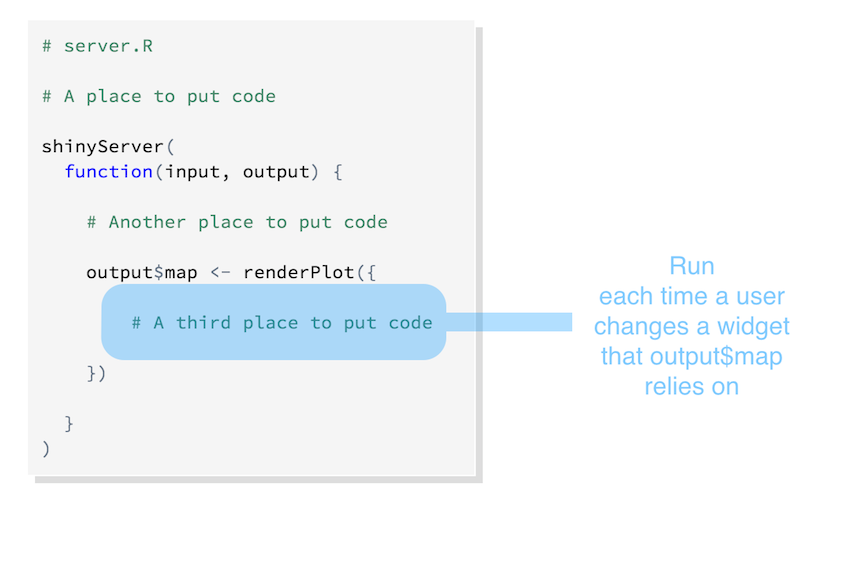
\includegraphics[scale=0.4]{place-of-code}

\begin{enumerate}
\item Le premier endroit n'est exécuté qu'au lancement de l'application, une seule fois.
\item Le deuxième est exécuté à chaque arrivée d'un nouvel utilisateur (?)
\item Le troisième est exécuté à chaque fois que l'utilisateur modifie un widget, soit, très, très, souvent.
\end{enumerate}

L'outil \verb!switch! est cool : 
\begin{verbatim}
data <- switch(input$var, 
        "Percent White" = counties$white,
        "Percent Black" = counties$black,
        "Percent Hispanic" = counties$hispanic,
        "Percent Asian" = counties$asian)
\end{verbatim}
Permet de faire un «mappage» entre différents éléments.
On peut également appeler une fonction avec une liste d'argument en utilisant \verb!do.call! ce qui permet de créer un code plus compact.

\begin{verbatim}
library(maps)
library(mapproj)
counties <- readRDS("data/counties.rds")
source("helpers.R")
    
    
shinyServer(
  function(input, output) {
    output$map <- renderPlot({
      args <- switch(input$var,
        "Percent White" = list(counties$white, "darkgreen", "% White"),
        "Percent Black" = list(counties$black, "black", "% Black"),
        "Percent Hispanic" = list(counties$hispanic, "darkorange", "% Hispanic"),
        "Percent Asian" = list(counties$asian, "darkviolet", "% Asian"))
        
      args$min <- input$range[1]
      args$max <- input$range[2]
  
      do.call(percent_map, args)
    })
  }
)
\end{verbatim}
\section{Expressions réactives : reactive expressions}
Commençons par un exemple :
\begin{verbatim}
dataInput <- reactive({
  getSymbols(input$symb, src = "yahoo", 
    from = input$dates[1],
    to = input$dates[2],
    auto.assign = FALSE)
})
\end{verbatim}
Ici on pourra désormais accèder au données renvoyées par \verb!getSymbols! en utilisant \verb!dataInput()!. \\
Les expressions réactives sont plus «intelligentes» que les fonctions classiques de R. Elle «cachent» leurs contenu et savent quand il est nécessaire de le mettre à jour. \\
Il ne faut les appeler que dans d'autres expressions réactives ou bien des fonctions \verb!render*!. \\
On peut les utiliser pour séparer la mise à jour en fonction de la variable qui a changée. Un seul bloc \verb!render*! se mettra par exemple à jour dès qu'un input a été changé, n'importe lequel. En revanche en utilisant plusieurs expressions réactives on peut séparer et ne pas forcément tout recalculer si A ET B ont changé, mais recalculer seulement une partie si seulement A a changé (idem avec seulement B).
\end{document}